\documentclass[a4paper, 12pt]{article}
\usepackage[utf8]{inputenc}
\usepackage[T1]{fontenc}
\usepackage[english]{babel}
\usepackage{booktabs}
%% Sets page size and margins
\usepackage[a4paper,top=2cm,bottom=2cm,left=2.5cm,right=2.5cm,marginparwidth=1.75cm]{geometry}
\usepackage{setspace}
\usepackage{float}

% Load packages
\usepackage[style=authoryear-ibid, backend=biber]{biblatex}
\usepackage{graphicx}
\usepackage{xcolor, soul}
\usepackage[hidelinks]{hyperref}
\usepackage{multirow}
\usepackage{rotating}
\usepackage{subfiles}
\usepackage{csquotes}

\usepackage{makecell} % for more vertical space in cells
\setcellgapes{5pt}

\usepackage{pdfpages}

\DefineBibliographyStrings{english}{%
  bibliography = {References},
}

\addbibresource{bibliography.bib}

% Dane magistranta:
\author{Szymon Socha, Piotr Wójcik}

% Dane magistrantów:
%\autor{Autor Zerowy}{342007}
%\autori{Autor Pierwszy}{342013}
%\autorii{Drugi Autor-Z-Rzędu}{231023}
%\autoriii{Trzeci z Autorów}{777321}
%\autoriv{Autor nr Cztery}{432145}
%\autorv{Autor nr Pięć}{342011}

\title{Should You Care about Tools in Fake News Detection? A Comparative Study of Cutting-Edge Embedding Methods and Classification Algorithms}

% miesiąc i~rok:
\date{}

% Tu jest dobre miejsce na Twoje własne makra i~środowiska:
\newtheorem{defi}{Definicja}[section]

% koniec definicji

\begin{document}

% \newpage % strona tytulowa
% \thispagestyle{empty}
% \
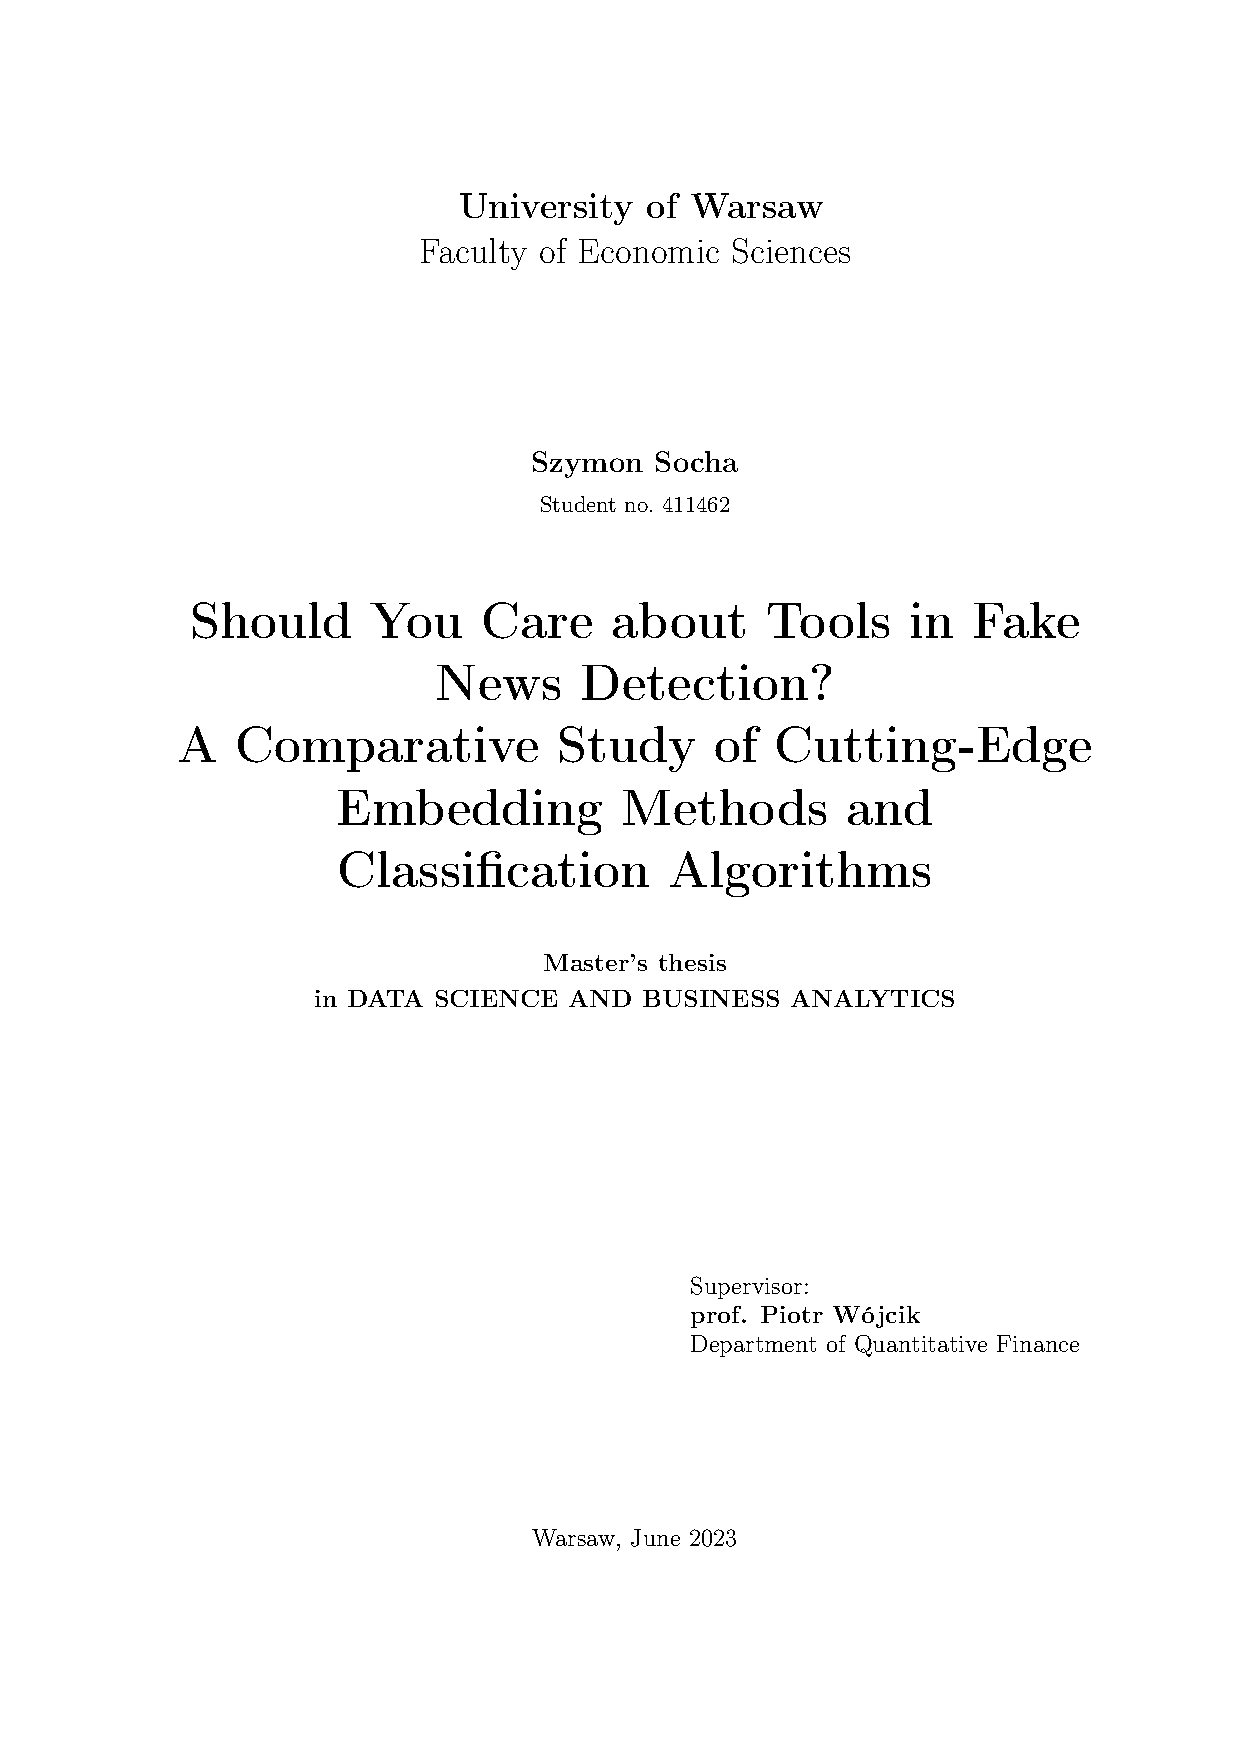
\includepdf{title.pdf}

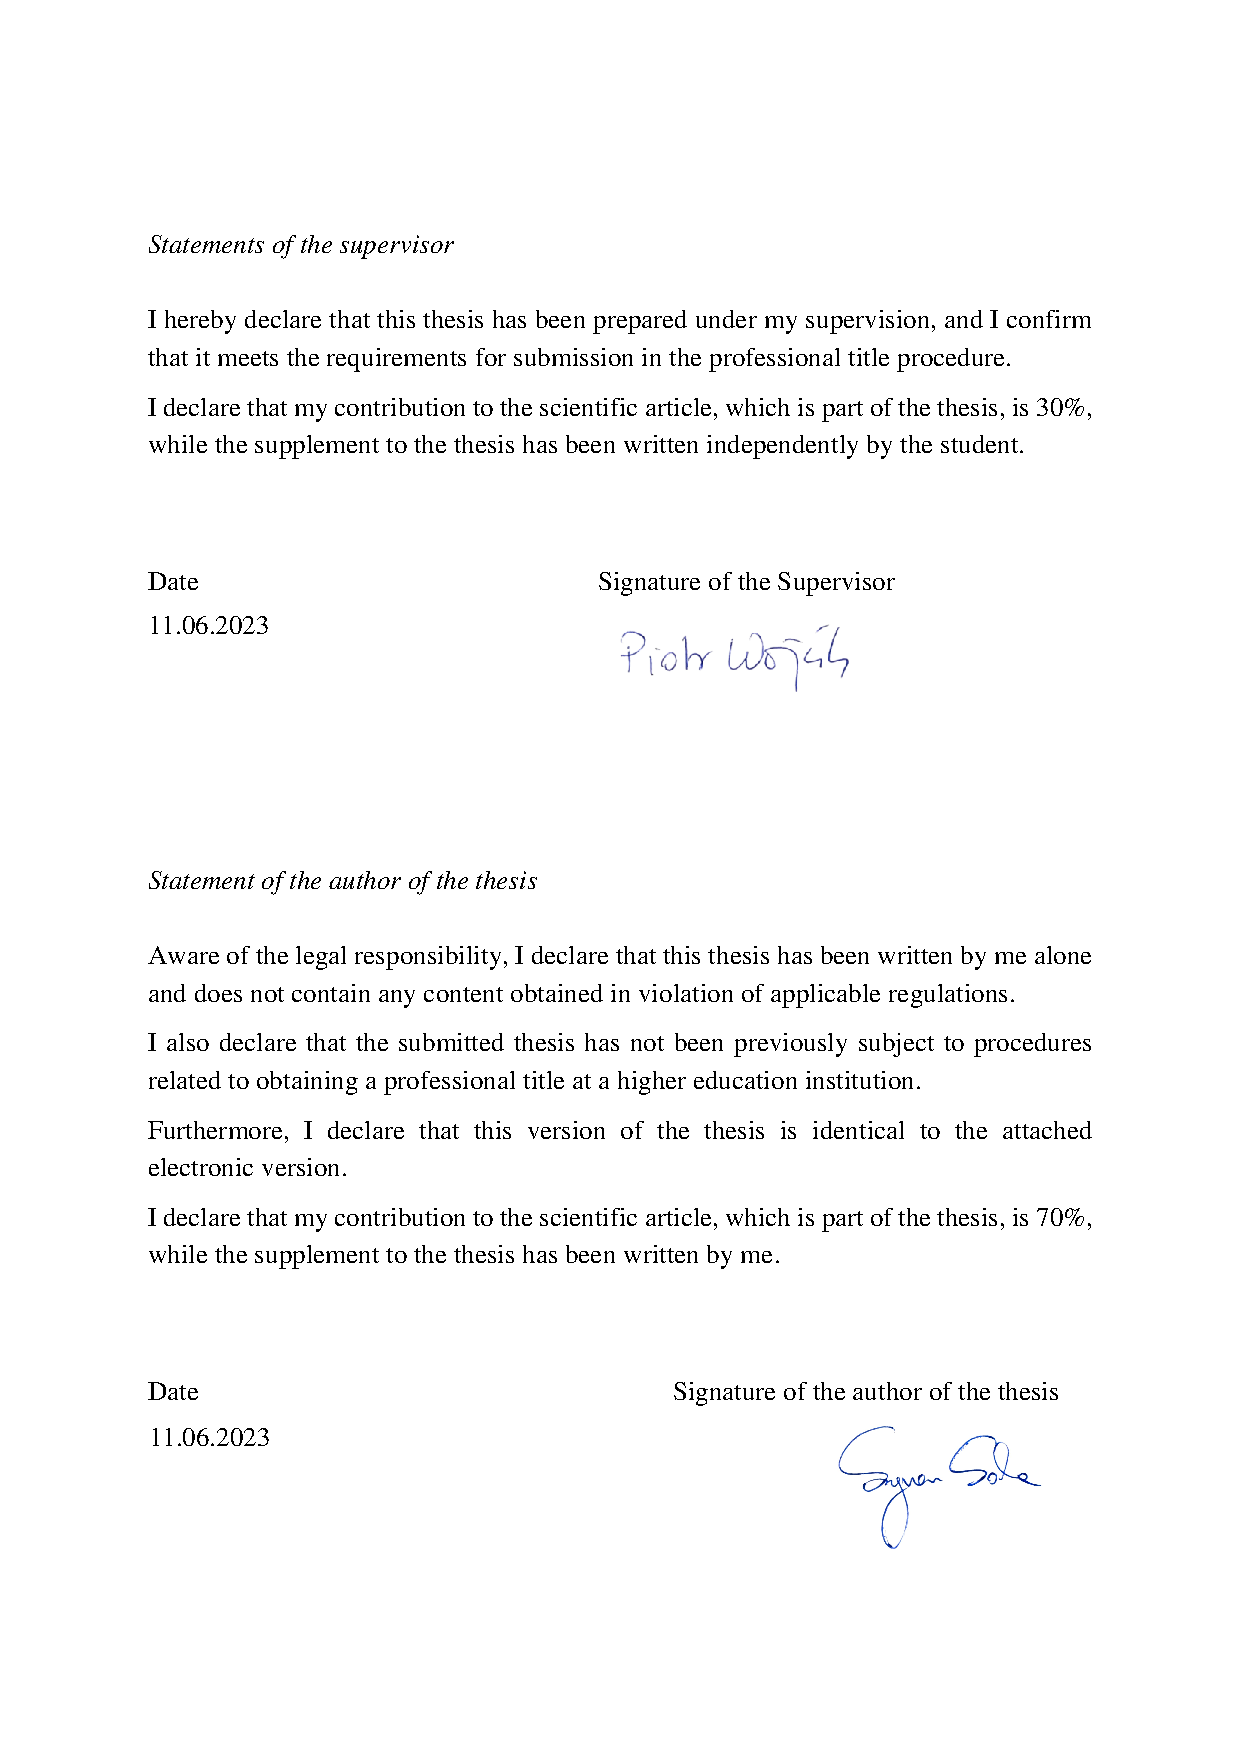
\includepdf{oswiadczenie_SZSocha_signed.pdf}
% \newpage % strona ze streszczeniem i inne
% \thispagestyle{empty}
% \vspace*{\fill}
% \noindent\textit{Statements of the supervisor}
% \vspace{0.5cm}

% \noindent I hereby declare that this thesis has been prepared under my supervision, and I confirm that it meets the requirements for submission in the professional title procedure.
% \vspace{0.25cm}

% \noindent I declare that my contribution to the scientific article, which is part of the thesis, is 30\%, while the supplement to the thesis has been written independently by the student.
% \vspace{2cm}

% \noindent Date \hspace{8cm}  Signature of the supervisor
% \vspace{3cm} 

% \noindent\textit{Statement of the author of the thesis}
% \vspace{0.5cm}

% \noindent Aware of the legal responsibility, I declare that this thesis has been written by me alone and does not contain any content obtained in violation of applicable regulations.
% \vspace{0.25cm}

% \noindent I also declare that the submitted thesis has not been previously subject to procedures related to obtaining a professional title at a higher education institution.
% \vspace{0.25cm}

% \noindent Furthermore, I declare that this version of the thesis is identical to the attached electronic version.
% \vspace{0.25cm}

% \noindent I declare that my contribution to the scientific article, which is part of the thesis, is 70\%, while the supplement to the thesis has been written by me.
% \vspace{2cm}

% \noindent Date \hspace{8cm}  Signature of the author of the thesis
% \vspace{2cm} 
% \vspace*{0.7\fill}
% \vfill

% \newpage % strona ze streszczeniem i inne
% \thispagestyle{empty}
% \
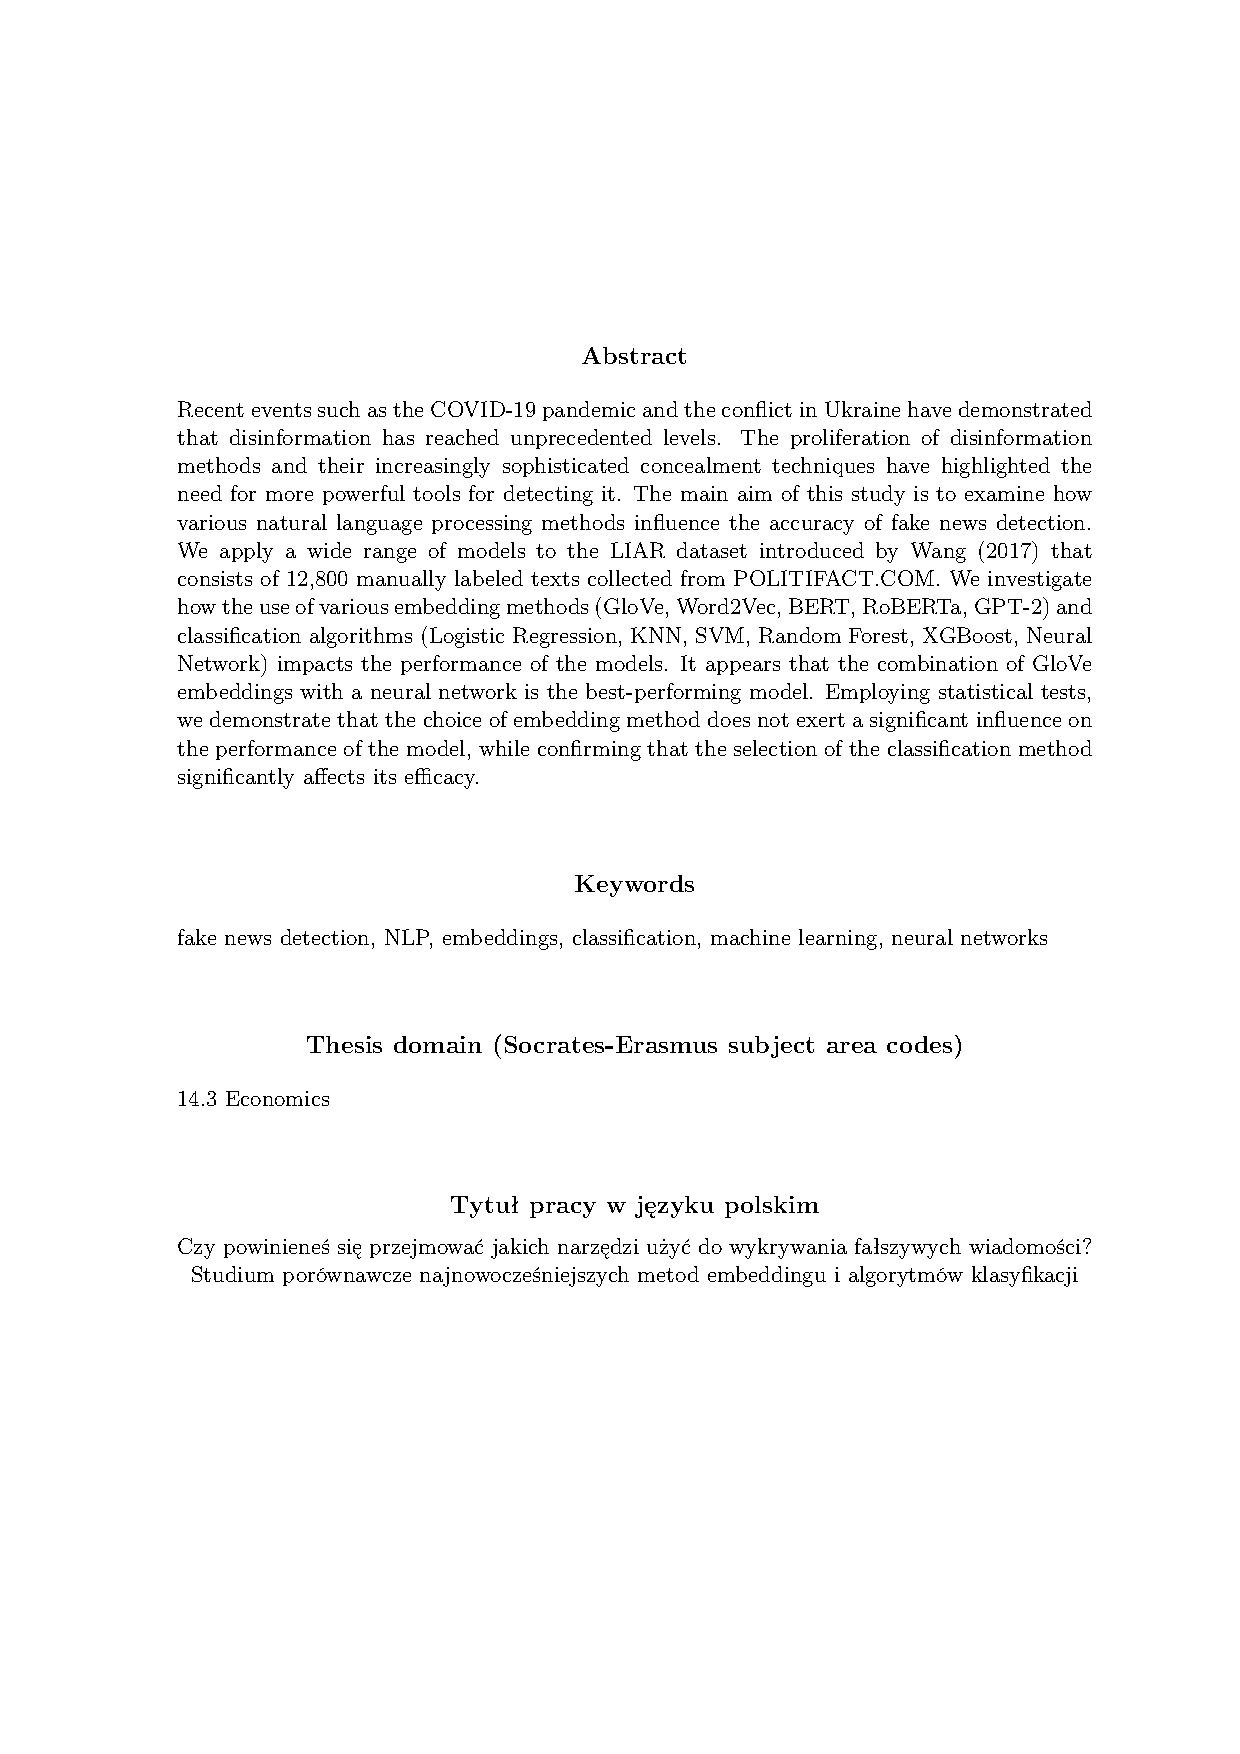
\includepdf{streszczenie.pdf}

\newpage
\vspace*{\fill}
\tableofcontents
\vspace*{\fill}
\thispagestyle{empty}

\newpage
\thispagestyle{empty}
\vspace*{\fill}
\begin{center}
    \Huge{\textbf{Scientific Article}}
\end{center}
\vspace*{0.7\fill}
\vfill

\newpage % strona ze streszczeniem i inne
\thispagestyle{empty}
\
\newpage

\clearpage
\pagenumbering{arabic}
\newpage

\maketitle

%tu idzie streszczenie na strone poczatkowa
\begin{abstract}
    Recent events such as the COVID-19 pandemic and the conflict in Ukraine have demonstrated that disinformation has reached unprecedented levels. The proliferation of disinformation methods and their increasingly sophisticated concealment techniques have highlighted the need for more powerful tools for detecting it. 
    The main aim of this study is to examine how various natural language processing methods influence the accuracy of fake news detection. We apply a wide range of models to the LIAR dataset introduced by Wang (2017) that consists of 12,800 manually labeled texts collected from POLITIFACT.COM. We investigate how the use of various embedding methods (GloVe, Word2Vec, BERT, RoBERTa, GPT-2) and classification algorithms (Logistic Regression, KNN, SVM, Random Forest, XGBoost, Neural Network) impacts the performance of the models. It appears that the combination of GloVe embeddings with a neural network is the best-performing model. Employing statistical tests, we demonstrate that the choice of embedding method does not exert a significant influence on the performance of the model, while confirming that the selection of the classification method significantly affects its efficacy.
\end{abstract}

\textbf{Keywords}: fake news detection, NLP, embeddings, classification, machine learning, neural networks


\linespread{1.5}

\section*{Introduction}
\subfile{sections/section1_introduction_article}

\section{Related Work}\label{r:related_work}

\subfile{sections/section2_relatedwork_article}

\section{Methodology}\label{r:methodology}
\subfile{sections/section3_methodology_article}
\subfile{sections/section3a_results_article}

\section*{Conclusion}\label{r:conclusion}
\subfile{sections/section4_conclusion}

\linespread{1.2}

\printbibliography

\newpage
\appendix

\linespread{1.5}

\section{Text pre-processing}\label{r:text_preparation}
\subfile{appendix/text_preparation}

\section{Extended results}\label{r:extended_results}
\subfile{appendix/extended_results}

\newpage
\listoffigures
\listoftables

%\begin{thebibliography}{99}
%\addcontentsline{toc}{chapter}{Bibliography}
%\printbibliography[heading=bibintoc]

\end{document}

%%% Local Variables:
%%% mode: latex
%%% TeX-master: t
%%% coding: latin-2
%%% End:
